\chapter{Versuchergebnisse}
\label{chap:versuchergenisse}

% ----------------------------------------
% Sec: Vergleichsmessung von modifizierten Teilen
% ----------------------------------------
\section{Vergleichsmessung von modifizierten Teilen}
\label{sec:vergleichsmessung_von_difizierten_Teilen}

Zur Überprüfung der Funktion des neuen Systems, werden die Schmierfilmhöhen gegenübergestellt, die einerseits mit den modifizierten und anderseits mit den originalen Teilen (Kugel + Support) gemessen werden.
Außerdem werden diese Messergebnisse mit den von theoretischer Berechnung verglichen.

Die Vergleichsmessung wird mit dem Mineralöl \textit{FVA 3} bei der Temperatur von \SI{40}{\degreeCelsius} und der Last von \SI{20}{\N} durchgeführt (siehe Abbildung~\ref{fig:vergleichsmessung}).
Man kann hier sehen, dass das neue System gut funktioniert, die Messwerte liegen nah zu einander.

% ----------------------------------------
% Fig: Vergleichsmessung von neuer Kugel + neuer Scheibe,
% neuer Kugel + alte Scheibe und theoretische Filmdicke
% ----------------------------------------
\begin{figure}[htb]
    \centering
    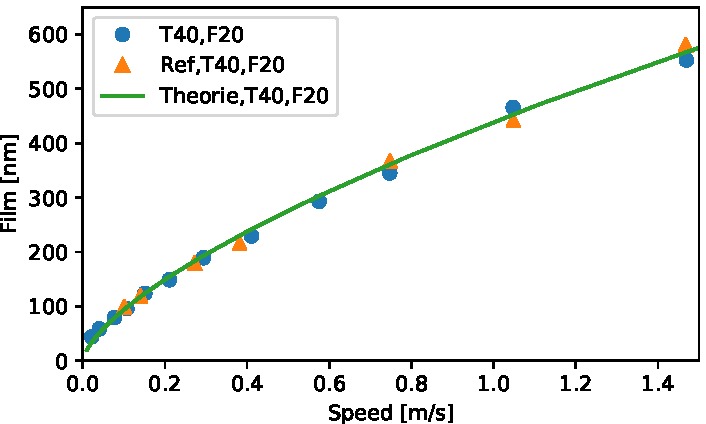
\includegraphics[]{./images/vergleichsmessung_T40_F20_FVA3.pdf}
    \caption{Filmdicke von zwei Konfigurationen --- neue Kugel + neue Scheibe (rund); originale Teile (dreieckig); rechnerische Filmdicken (gerade) --- mit dem Öl \textit{FVA 3} bei $T =$ \SI{40}{\degreeCelsius} und $F =$ \SI{20}{\N}}
    \label{fig:vergleichsmessung}
\end{figure}

% ----------------------------------------
% Sec: Störkapazitätmessung
% ----------------------------------------
\section{Störkapazitätsmessung}
\label{sec:stoerkapazitaetsmessung}

Da die kapazitiven Messungen von elektrischen Störungen, die von Elektrogeräten im Labor enstehen, sehr empfindlich sind, werden die Kabel so kurz wie möglich gehalten.
Alle elektronischen Anschlüsse und Bauteile werden nah zu einander auf einer Platine gebaut.
Trotz dieser Maßnahmen kann man leider nie die Störungen eliminieren.
Aus diesem Grund wird diese ungewünschte Größen bzw. Störkapazität bei stationären Zustand, mit alle benötigen Geräten angemacht werden, gemessen.
Diese beträgt ca. \SI{89}{\pico\farad} und wird danach von den Messergebnissen abgezogen.
Abbildung~\ref{fig:vergleichsmessung} zeigt die Bestimmung der Störkapazität an.

% ----------------------------------------
% Fig: Background capacitance
% ----------------------------------------
\begin{figure}[htb]
    \centering
    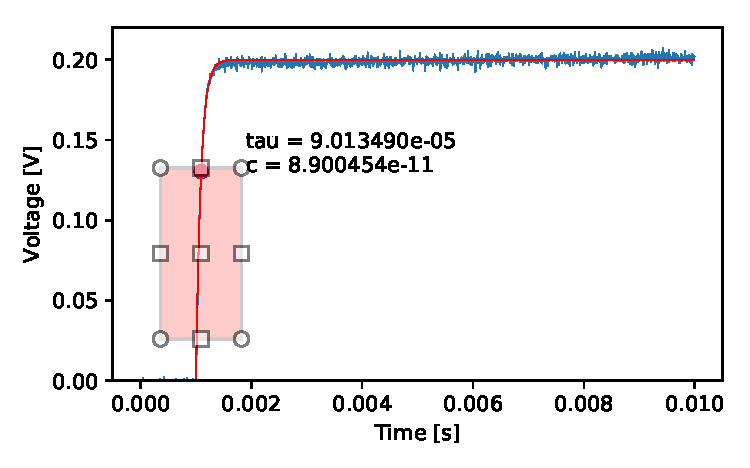
\includegraphics[]{./images/background_capacitance.pdf}
    \caption{Bestimmung der Störkapazität bevor einem Versuch: Messdaten (blau); angepasste Kurve (rot)}
    \label{fig:background_capacitance}
\end{figure}

% ----------------------------------------
% Sec: Kapazitätsmessung für EHD-Punktkontakt
% ----------------------------------------
\section{Kapazitätsmessung für EHD-Punktkontakt}
\label{sec:kapazitaetsmessung_punktkontakt}

Abbildung~\ref{fig:cap_vs_speed_dif_temp_meas} gibt einen Einblick in das Verhalten der kapazitiven Messwerte bei einer Variation der Temperaturen.
Der Haupttrend, der hier beobachtet werden kann, ist die Abnahme der Kapazität bei der Zunahme der Temperatur.
Dieses Phänomen stimmt mit der Analyse im Abschnitt~\ref{sec:versuchsplanung} ab, da die Filmdicke mit steigender Temperatur abnimmt.

% ----------------------------------------
% Fig: Kapazitätsmessung bei verschiedenen Temperaturen
% ----------------------------------------
\begin{figure}[htb]
    \centering
    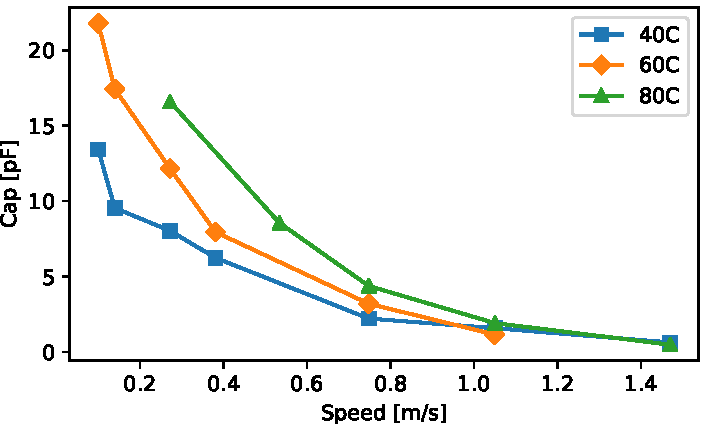
\includegraphics[]{./images/cap_vs_speed_dif_temp_meas.pdf}
    \caption{Kapazitätsmessung für das Mineralöl \textit{FVA 3} bei unterschiedlichen Temperaturen und einer Last von \SI{20}{\N}}
    \label{fig:cap_vs_speed_dif_temp_meas}
\end{figure}

Der Zusammenhang zwischen der gemessenen Kapazitäten und der aufgenommenen Schmierfilmhöhen bei einzelner Versuchstemperatur wird in Abbildung~\ref{fig:cap_meas_cap_theo_40C},~\ref{fig:cap_meas_cap_theo_60C} und~\ref{fig:cap_meas_cap_theo_80C} dargestellt.
Zum Vergleichszweck werden auch die rechnerischen Kapazitäten anhand den Schmierfilmdicken ins Diagramm eingetragen.

Man kann hier sehen, dass die gemessenen Werte relativ nah zu den rechnerischen bei niedrigen Geschwindigkeiten liegen.
Bei größeren Filmhöhen weichen die beiden leider von einander ab.
Eine Erklärung dafür wäre, dass die Kapazität bei einem dickeren Film so niedrig ist, sodass eine fehlerfrei Auswertung von Messwerten nicht vermeidbar ist.
Es kann auch sein, dass die Motoren und die elektronische Einheit bei hoher Belastung mehr Störungen abgeben.
Das heißt, dass die Störkapazität variieren kann.
Da die Messwerte von der Störkapazität, die beim Stillstand gemessen wird, abgezogen werden, könnte es die Fehler bei der Auswertung produzieren.

% ----------------------------------------
% Fig: Kapazitätsmessung bei 40C
% ----------------------------------------
\begin{figure}[htb]
    \centering
    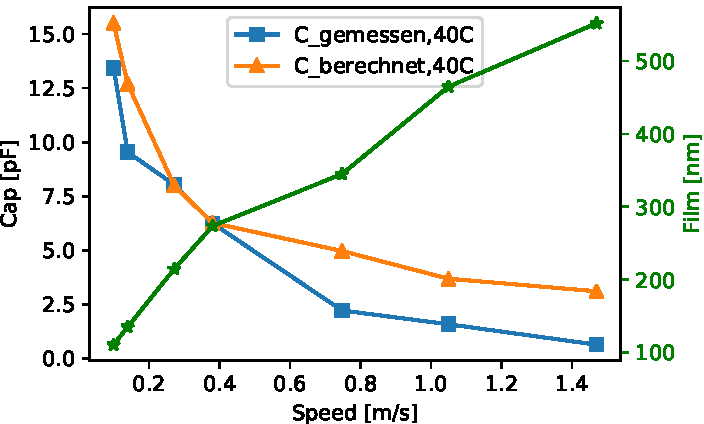
\includegraphics[]{./images/cap_theo_meas_vs_speed_40C.pdf}
    \caption{gemessenen Kapazitäten im Vergleich mit rechnerischen bei aufgenommen Filmhöhen von dem Öl \textit{FVA 3} bei $T =$ \SI{40}{\degreeCelsius} und $F =$ \SI{20}{\N}}
    \label{fig:cap_meas_cap_theo_40C}
\end{figure}

% ----------------------------------------
% Fig: Kapazitätsmessung bei 60C
% ----------------------------------------
\begin{figure}[htb]
    \centering
    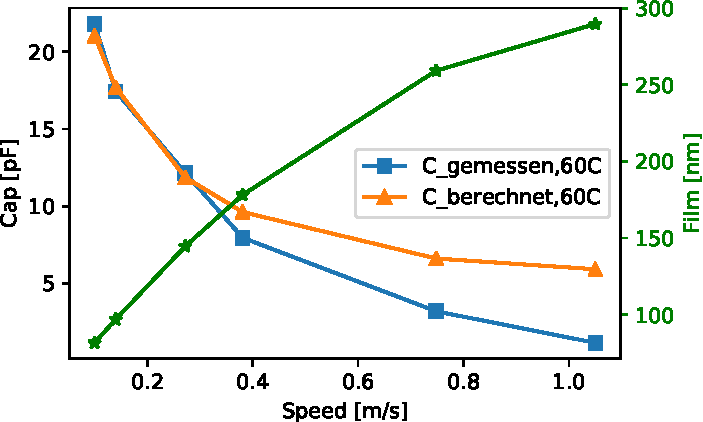
\includegraphics[]{./images/cap_theo_meas_vs_speed_60C.pdf}
    \caption{gemessenen Kapazitäten im Vergleich mit rechnerischen bei aufgenommen Filmhöhen von dem Öl \textit{FVA 3} bei $T =$ \SI{60}{\degreeCelsius} und $F =$ \SI{20}{\N}}
    \label{fig:cap_meas_cap_theo_60C}
\end{figure}

% ----------------------------------------
% Fig: Kapazitätsmessung bei 80C
% ----------------------------------------
\begin{figure}[htb]
    \centering
    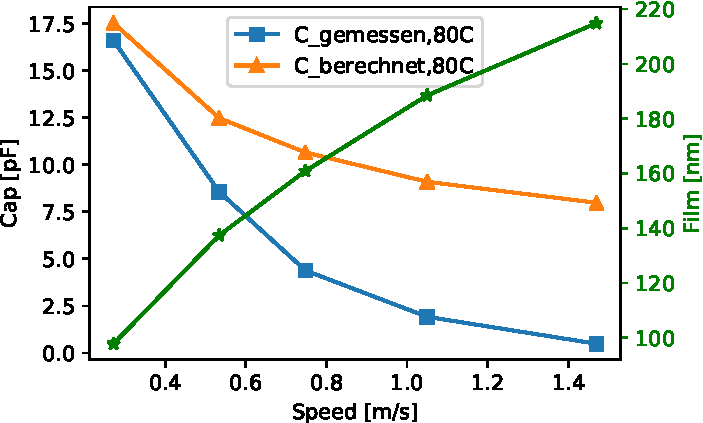
\includegraphics[]{./images/cap_theo_meas_vs_speed_80C.pdf}
    \caption{gemessenen Kapazitäten im Vergleich mit rechnerischen bei aufgenommen Filmhöhen von dem Öl \textit{FVA 3} bei $T =$ \SI{80}{\degreeCelsius} und $F =$ \SI{20}{\N}}
    \label{fig:cap_meas_cap_theo_80C}
\end{figure}

% ----------------------------------------
% Sec: Einschränkung des Systems und Verbesserungsvorschlag
% ----------------------------------------
\section{Einschränkung des Systems und Verbesserungsvorschläge}
\label{sec:einschraenkung_des_systems_und_verbesserungsvorschlaege}

Da es hier um einzelnen EHD-Kontakt handelt, ist der messbare Kapazität-Bereich sehr klein (theoretisch unter \SI{18}{\pico\farad}).
Die Störung von der Umgebung und der Kabeln beträgt allein schon ca. \SI{89}{\pico\farad}.
Deswegen ist es sinnvoll, die Kabel und alle elektronischen Geräte von der Messkette gegen äußerlichen Störungen abzuschirmen.
Die elektronischen Bauteile (Widerstand, Kabel-Anschlüsse) sollten auf einer Platine gebaut und so nah wie möglich zu der Messkarte platziert werden.
Abbildung~\ref{fig:ebox_fuer_mobil_und_lcr_meter} zeigt die Konstruktion von den E-Box, wo die elektronischen Bauteile kompakt aufgebaut werden.

% ----------------------------------------
% Fig: Elektronischer E-Box
% ----------------------------------------
\begin{figure}[htb]
    \centering
    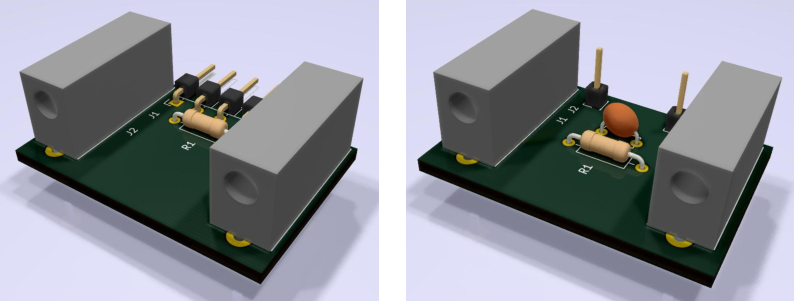
\includegraphics[]{./images/ebox_ladekurve_lcr-meter.pdf}
    \caption{E-Box, wo die elektronischen Bauteile und Kabel-Anschlüsse auf einer Platine gelötet werden: Links für das mobiles Messsystem, rechts für das LCR-Meter}
    \label{fig:ebox_fuer_mobil_und_lcr_meter}
\end{figure}

Mit einem Vorwiderstand $R_V =$ \SI{1012.7}{\ohm} kann die Messkarte USB-6211 von \textit{NI} (Abtastrate \SI[per-mode=symbol]{250}{\kilo\sample\per\second}) im besten Fall, die Vollladung eines Kondensator mit $C =$ \SI{0.788}{\pico\farad} messen.
Um die Auflösung zu erhöhen, kann man den großeren Wert des Vorwiderstands nehmen.
Allerdings ist es unerwünscht, da das Auflade- und Entladeverhalten des Systems verändert wird.
Eine bessere Lösung wäre, eine andere Messkarte, die schnellere Abtastrate hat, zu verwenden.

Die Chromschicht auf der neuen Glasscheibe ist ca. \SI{600}{\nm} dick.
Obwohl dieses gut für Reduzierung des Eigenwiderstands der Schicht ist, tritt es wegen ihrer Dicke einige Probleme auf.
Da die Chromschicht und das Glas unterschiedlichen Wärmeausdehnungskoeffizienten haben, ist die Beschichtung schon bevor dem Versuch bei Lagerung beschädigt worden.
Auf einigen Stellen der Scheibe werden die Beschichtung aus der Glasoberfläche abgebrochen (siehe Abbildung~\ref{fig:beschaedige_glasscheibe}).
Da die Haftung der Chromschicht auf dem Glas nicht so gut ist, entsteht eine Rille sofort nach einer Messung.
Diese beschränkt die befahrenden Spuren und reduziert die Lebensdauer der Scheibe enorm.
Ein Vorschlag wäre, eine dünnere Chromschicht und bessere Vorbereitung der Glasoberfläche zu haben.

% ----------------------------------------
% Fig: Beschädige Glasscheibe
% ----------------------------------------
\begin{figure}[htb]
    \centering
    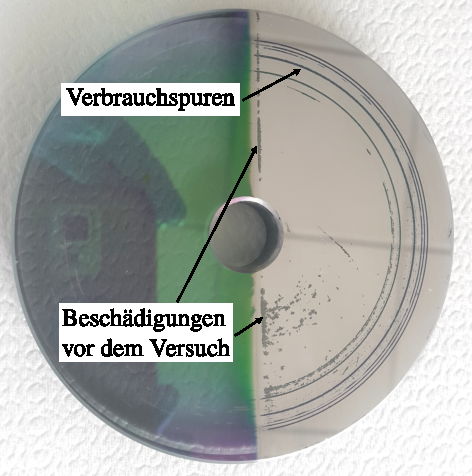
\includegraphics[]{./images/beschaedige_scheibe.pdf}
    \caption{Die beschädige Glasscheibe mit deutlich erkennbare Verbrauchspuren}
    \label{fig:beschaedige_glasscheibe}
\end{figure}
